\chapter{Uvedenie do problematiky a súčasný stav}

\label{kap:uvod_teoria}

\section{Spôsob merania}
Dáta sú výsledkom dlhodobého merania. Vrámci merania sa v pravidelných intervaloch opakovane volali príkazy \lstinline{ping} a \lstinline{traceroute} na postupne 
rozširujúcu sa množinu IP adries. Výsledky meraní boli zapisované do PostgreSQL 8.1.9 databázy. Databáza má nasledujúcu štruktúru:

Tabuľka \lstinline{h_types} - Tabuľka obshujúca zoznam všetkých poznaných typov serverov na ktorých sa vykonávajú merania:
\begin{itemize}
    \item rank\_code - celé číslo, primárny kľúč
    \item rank\_description - reťazec - popis typu servera
    \item rank - reťazec - meno typu servera
\end{itemize}

Tabuľka \lstinline{hosts} - Tabuľka obshujúca zoznam všetkých IP adries na ktorých sa vykonávajú merania:
\begin{itemize}
    \item ip\_addr - IPV4 adresa vo formáte cidr, primárny kľúč - konkrétna hodnota IP adresy na ktorú sa riadok vzťahuje
    \item rank\_code - celé čislo, cudzí kľúč na tabuľku \lstinline{h_types} - typ servera na IP adrese
    \item enter\_date - časová pečiatka - dátum vloženia do zoznamu 
    \item source - reťazec - zdroj vloženia 
    \item comment - reťazec - komentár k IP adrese
    \item exclude - celé čislo - príznak, že daná adresa má byt vynechaná z merania
\end{itemize}

Tabuľka \lstinline{ping} - Tabuľka obshujúca záznamy o vykonaných meraniach dostupnosti a doby odozvy:
\begin{itemize}
    \item ip\_addr - IPV4 adresa vo formáte cidr, cudzí kľúč do tabuľky \lstinline{hosts} - konkrétna hodnota IP adresy na ktorú sa riadok vzťahuje
    \item ping\_rttmin - reálne číslo - minimálna nameraná doba odozvy v danom meraní
    \item ping\_rttmax - reálne číslo - maximálna nameraná doba odozvy v danom meraní
    \item ping\_rttavg - reálne číslo - priemerná nameraná doba odozvy v danom meraní
    \item ping\_rttmdev - reálne číslo - priemerná odchýlka doby odozvy v danom meraní
    \item ping\_ploss - celé číslo - počet percent stratených packetov alebo error kôd v prípade negatívnej hodnoty
    \item ping\_date - časová pečiatka - dátum a čas merania
\end{itemize}

Dátami v ďalších tabuľkách sa v tejto práci nebudeme zaoberať, ich štruktúru je možné vidieť v entitno-relačnom grafe \ref{obr:ent_rel_mfile}.
Dátový typ cidr je PostgreSQL dátový typ určený na ukladanie IP adries spolu s maskou podsiete. Pri ukladaní kontroluje, či sú za maskou len nulové 
bity, čím sa odlišuje od typu inet. Podporuje zoraďovanie podľa hodnoty a konverziu z reťazcovej reprezentácie \cite{cidr}. 

\begin{figure}
    \centerline{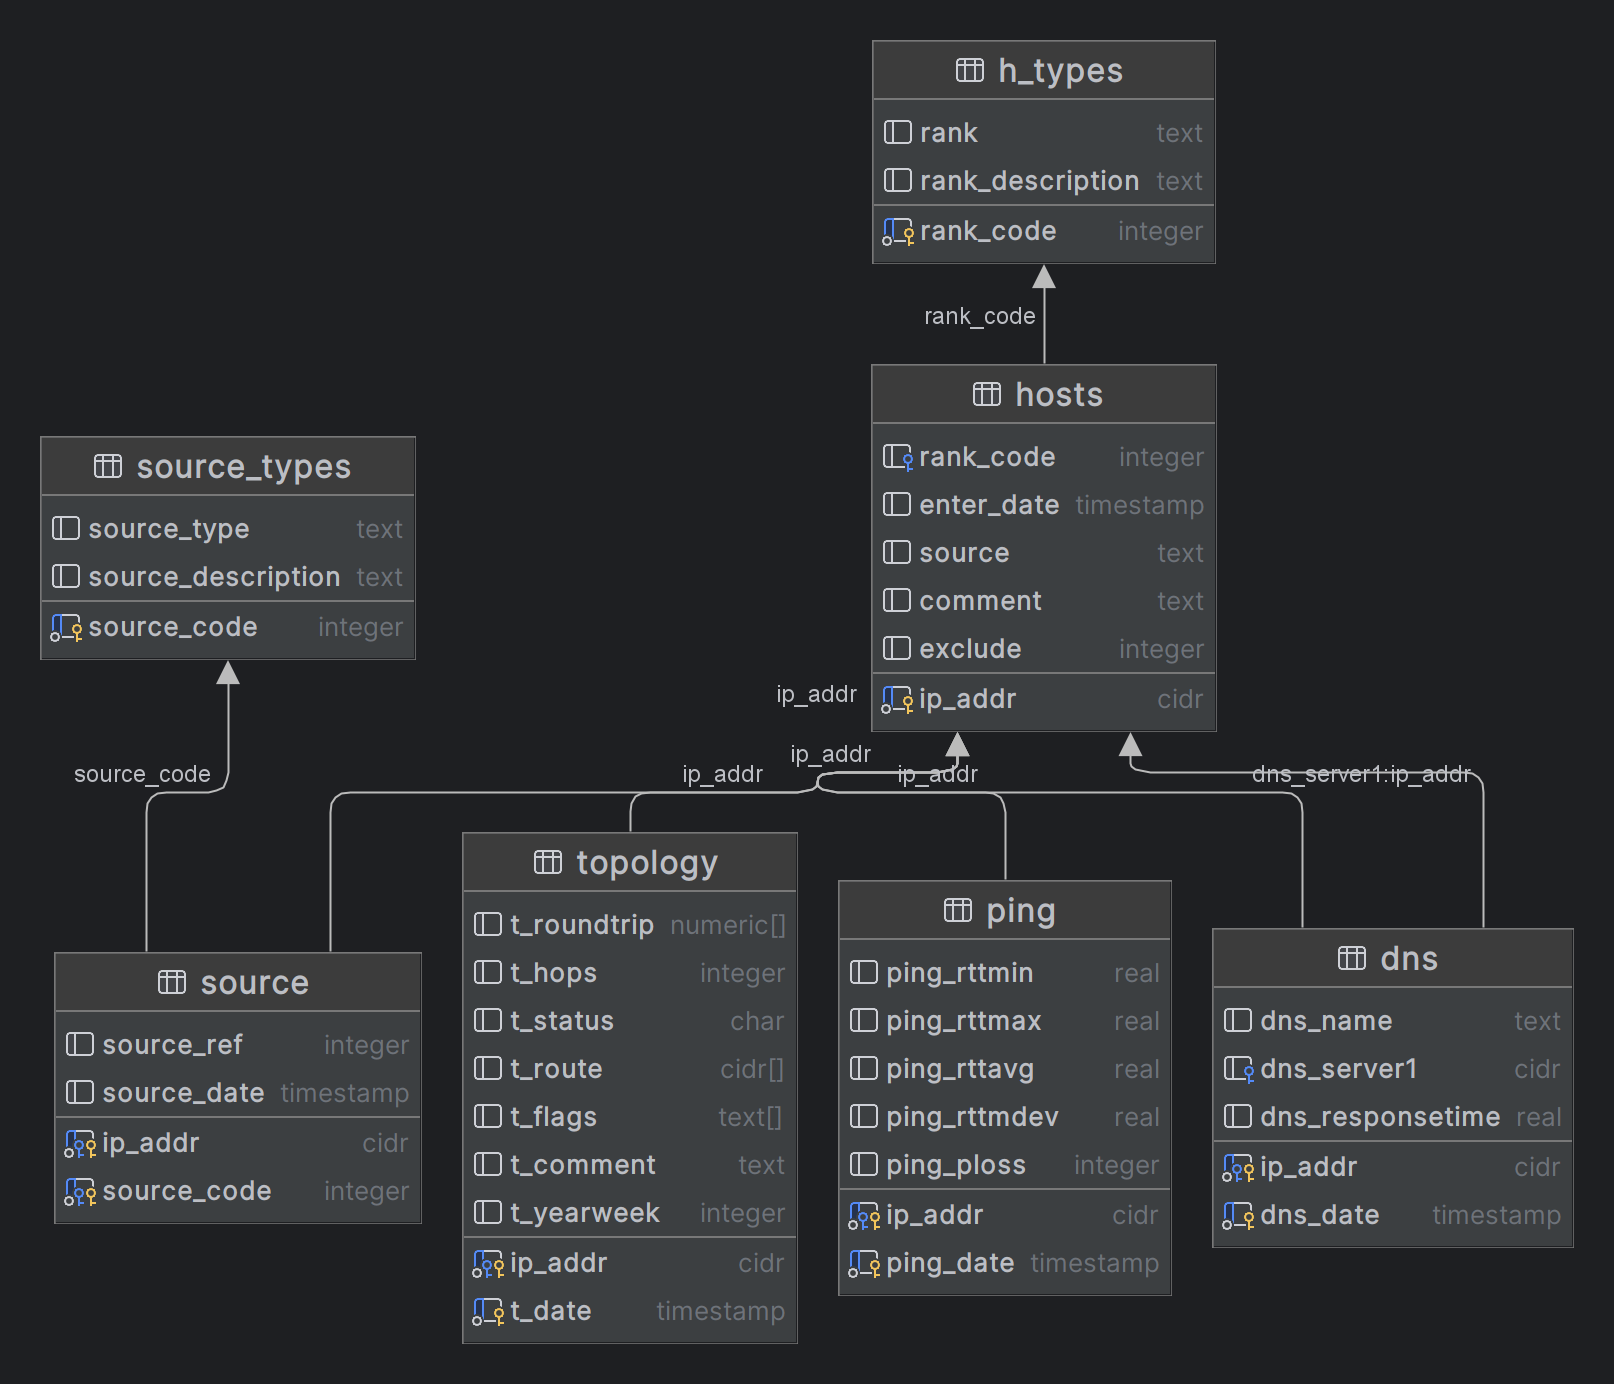
\includegraphics[width=0.8\textwidth]{images/mfile}}
    %popis obrazku
    \caption[Entitno-relačný diagram databázy s výsledkami meraní]{Entitno-relačný diagram databázy s výsledkami meraní}
    %id obrazku, pomocou ktoreho sa budeme na obrazok odvolavat
    \label{obr:ent_rel_mfile}
\end{figure}

Príkaz \lstinline{ping} zmeria dostupnosť a dobu odozvy servera. Príkaz pošle nastaviteľný počet paketov (predvolene 4) a sleduje, 
ktoré sa vrátia a za aký čas. Príkaz funguje v systéme Windows \cite{ping_windows} aj na Linuxových systémoch \cite{ping_linux}.
Príkaz \lstinline{traceroute} podobne ako \lstinline{ping} sleduje cestu paketov skrz uzly siete. Jeho výstupom je zoznam IP adries uzlov, ktorými paket prešiel 
na ceste k serveru s cieľovou IP adresou \cite{tracert}. 

\section{Prehľad súvisiacich projektov a existujúcich riešení}

\subsection{Projekty zaoberajúce sa dlhodobými meraniami internetu}

Analýzou databázy s existujúcimi dátami sa zaoberal Dennis Vita v ročníkovom projekte. Analyzoval kvalitu meraní a určoval množinu tzv. \uv{spoľahlivých} 
adries, teda adries, ktoré často odpovedajú \cite{vita_report}.

Dlhodobým meraním podobného charakteru a jeho vizualizácií sa venuje projekt CAIDA (Center for Applied Internet Data Analysis) na Univerzite 
v Kalifornii v San Diegu. V článku \cite{caida} sa zaoberajú dlhodobým meraním a vizualizáciou topológie siete. Podobnému meraniu a vizualizácii, 
ako napríklad zobrazeniu nameranej doby odozvy v mapách sa tiež venuje projekt RIPE Atlas \cite{atlas_ripe}.

\subsection{Riešenia zaoberajúce sa predspracovávaním a agregáciou údajov}

Dátový sklad (anglicky data warehouse) je systém, ktorý v pravidelných intervaloch zhromažďuje údaje z rôznych zdrojov, 
spracováva ich a vytvára medzi nimi vzťahy a tým pôsobí ako prehľadnejší zdroj užitočnejších dát ako pôvodné dáta \cite{data_warehouse}. 
Takéto riešenie je vhodné na analýzu veľkého množstva dát, akú budeme robiť my. Existuje niekoľko implemntácií 
dátových skladov, ako napríklad Snowflake, Google BigQuery alebo Amazon Redshift. My sa pokúsime o implementáciu vlastného jednoduchého 
dátového skladu určeného priamo namieru pre náš systém.